\documentclass[10pt,usenames,dvipsnames,t,leqno]{beamer}

\usetheme{metropolis}
\setbeamersize{text margin left=10pt,text margin right=10pt}
\usetikzlibrary{calc}
\usepackage{xcolor}
\usepackage{subfig}
\usepackage{multicol}
\definecolor{waterlooorange}{HTML}{FFD54F}
\definecolor{waterloodarkorange}{HTML}{E4B429}
\definecolor{waterlooyellow}{HTML}{FFEA3D}
\definecolor{mygray}{gray}{0.6}
\setbeamercolor{frametitle}{fg=black,bg=waterlooorange}
\setbeamercolor{progress bar}{fg=waterlooyellow,bg=mygray}
\setbeamercolor{background canvas}{bg=white}
\setbeamercolor{block body}{bg=waterlooorange!20,fg=black}
\setbeamercolor{block title}{bg=waterlooorange,fg=black}

\title{STAT 444 Final Project: Ames Housing Dataset Regression Analysis}
\author{Angelo Carreon, Hoseok Lee, Joy Chen, Steven Shen}
\date{} % Puts today's date

\setbeamercovered{invisible}

\begin{document}

\begin{frame}
\titlepage

\end{frame}

\begin{frame}{Exploratory Data Analysis and Preprocessing}
 
\textbf{Metadata:}
 
\begin{itemize}
\item In the original dataset, 82 covariates, $n=2930$ observations
\begin{itemize}
    \item 23 nominal, 23 ordinal, 14 discrete, 20 continuous
\end{itemize}
\item After data pre-processing, 19 covariates. 
    \begin{itemize}
    \item 7 nominal, 4 ordinal, 4 discrete, 4 continuous
    \end{itemize}
\item Response `SalePrice` was log-transformed for a more normal distribution.

\end{itemize}
 
\begin{figure}
    \centering
    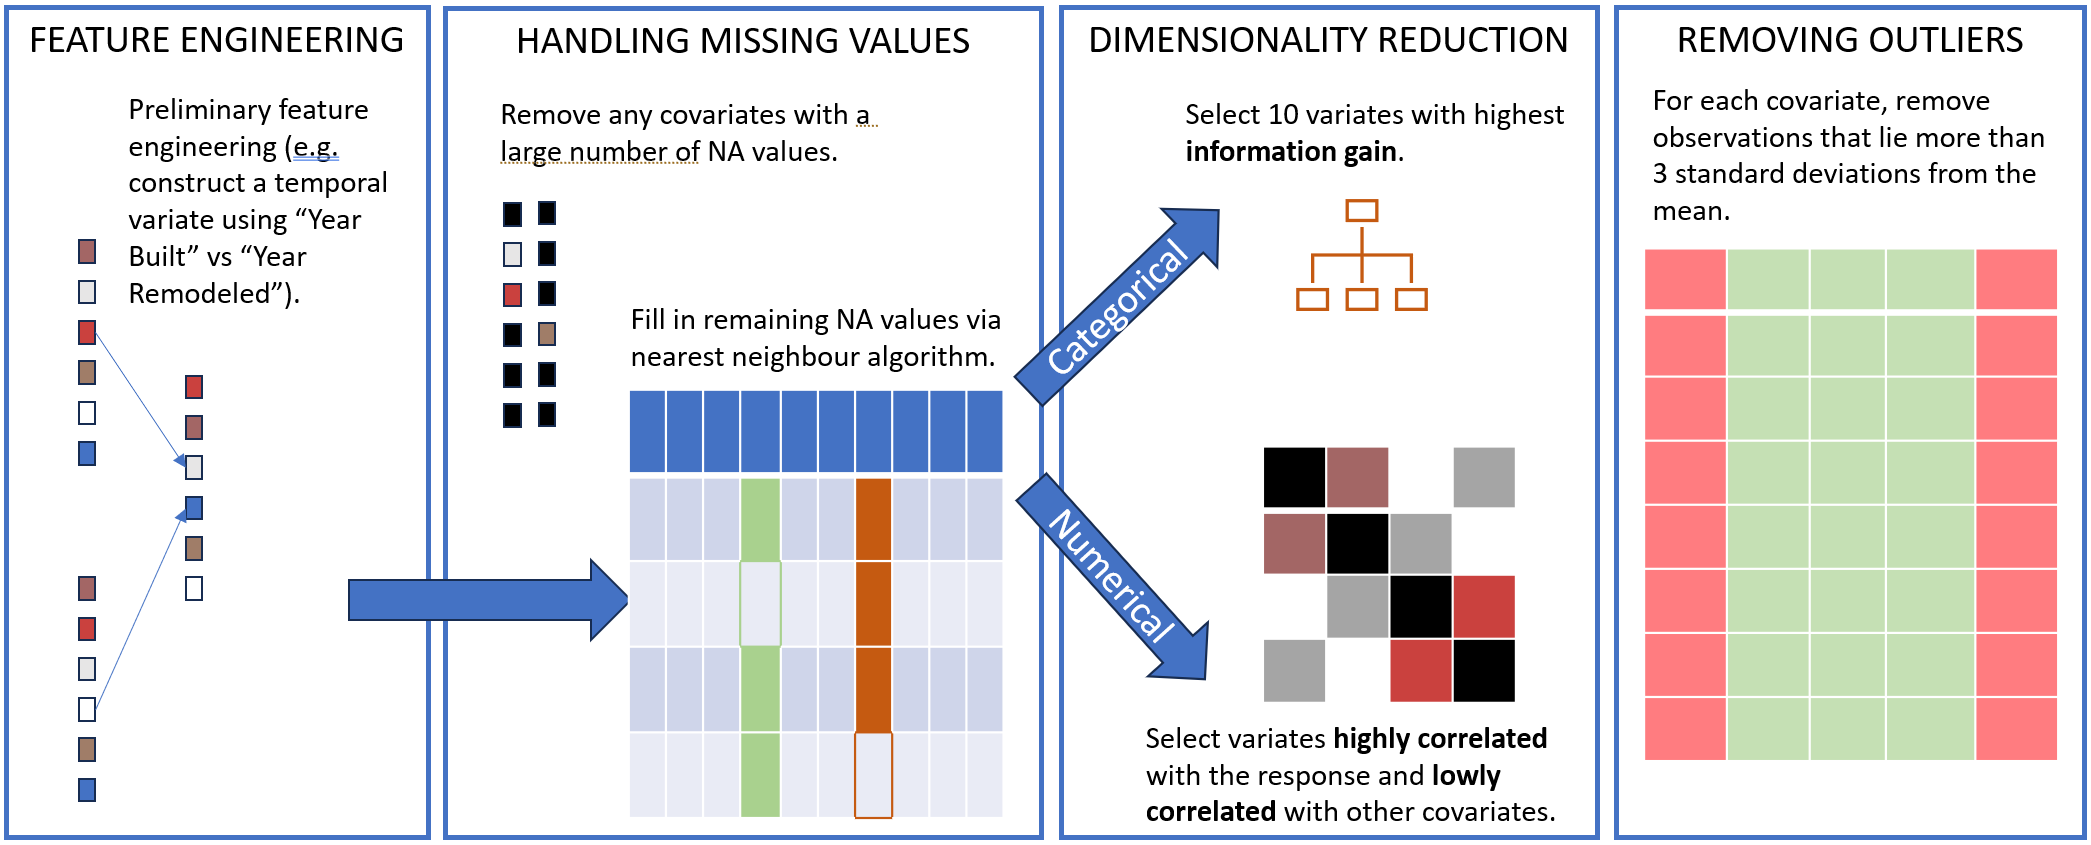
\includegraphics[width=0.9\linewidth]{EDA_PREPROCESSING.png}
\end{figure}
 
\end{frame}

\begin{frame}{Methods \& Models}
We compared four regression techniques to identify the most suitable model:
\begin{multicols}{2}
\begin{enumerate}
\itemsep0em
    \item Multiple Linear Regression
    \item Ridge
    \item Lasso
    \item GAM
\end{enumerate}
\end{multicols}
We assessed their performance using a 20-fold CV scheme, then tested their final performance under an 80:20 Train/Test split.
\begin{figure}
    \centering
    \subfloat[\centering CV Score]{{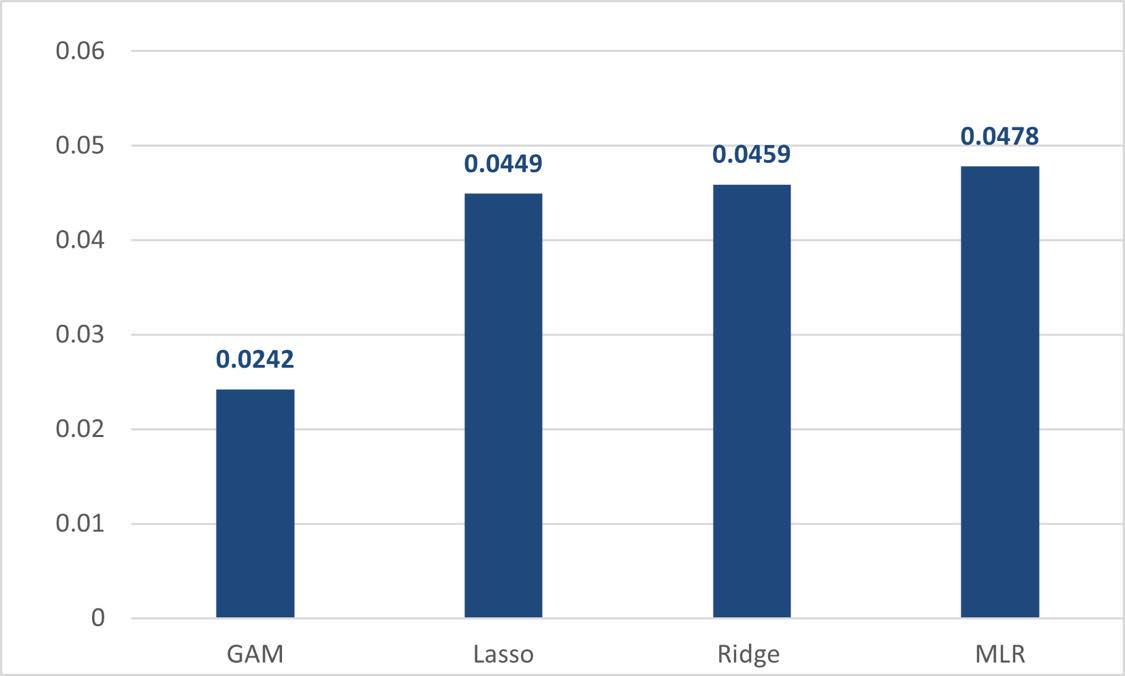
\includegraphics[width=5cm]{cv score.png} }}
    \qquad
    \subfloat[\centering Test Score]{{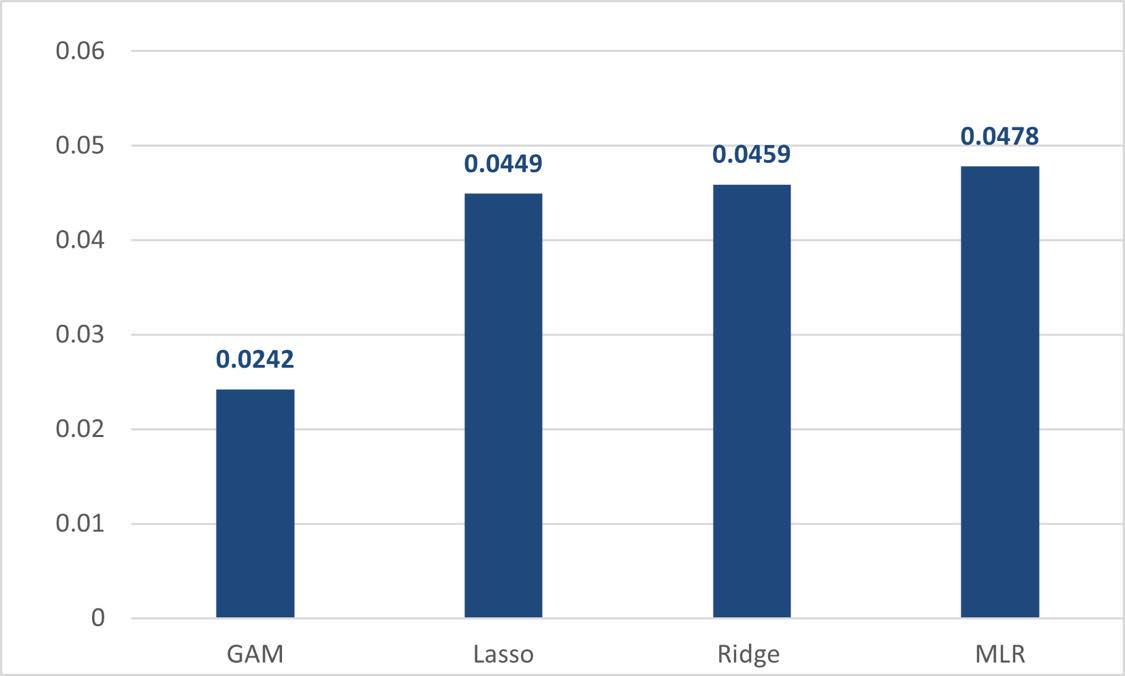
\includegraphics[width=5cm]{test score.png} }}
    \caption{Comparison of Model Performance}
    \label{fig:example}
\end{figure}
\end{frame}

\begin{frame}{Final Model Analysis: GAM Model}
The GAM model appeared to generate the best predictions. Why?
\begin{itemize}
\itemsep0em
\item Lots of non-linearity in the final list of (continuous) covariates
\item If it was addressed, we would expect better regression performance
\item In the end, our predictions were accurate with RMSE of approx. \$18,000
\end{itemize}
\begin{figure}
   \centering
    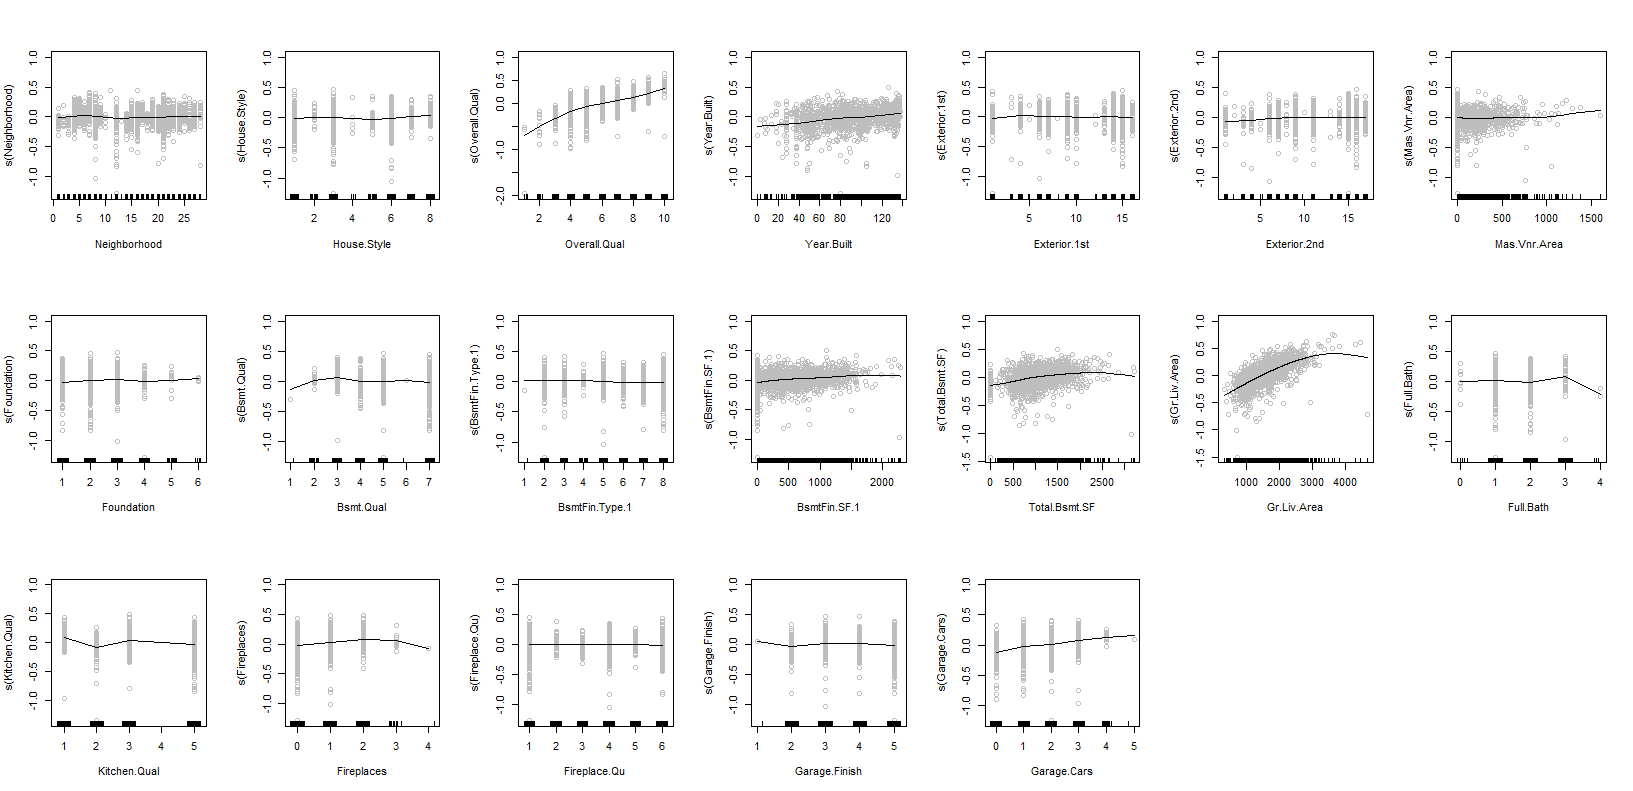
\includegraphics[width=0.8\linewidth]{gam_smooths.png}
    \caption{Fitted Smooths and Plotted Data of the final GAM model}
    \label{fig:example}
\end{figure}
\end{frame}

\end{document}
